\documentclass[a4paper]{article}
\usepackage[top=2cm]{geometry}
\usepackage{fontspec}
\setmainfont{Linux Libertine}
\input{ling_bib_conf.tex}
\addbibresource{cariban_references.bib}
\addbibresource{non_cariban_references.bib}
\usepackage{titlesec}
\input{booktabs_config}
\titleformat*{\section}{\normalsize\bfseries}
\usepackage{glossingtool}
\usepackage{graphicx}
\usepackage{subcaption}
\input{cariban_language_names.tex}
\usepackage[inline]{enumitem}
\newlist{inlinelist}{enumerate*}{1}
\setlist[inlinelist]{label={\alph*)}, itemjoin={{; }}, itemjoin*={{; and }}}
\newcommand{\emp}[1]{\textbf{#1}}
\usepackage{hyperref}
\usepackage[capitalise]{cleveref}
\providecommand{\goodtilde}{\char`~\xspace}


\begin{document}

	\begin{center}
		\bfseries
		\large{A second comparison of Cariban pronouns and deictics}\\
		\vspace{.05cm}
%		\normalsize{SUBTITLE}\\
		\vspace{.1cm}
		\normalfont

	\end{center}
%	Keywords: KEYWORDS
	\vspace{.4cm}
	
%	\begin{itemize}
%\item	\textcite[261]{meira2002first}: \gl{1+2} formatives may be old possessed nouns
%\item	\textcite[265]{meira2002first} tentatively reconstructs \rc{-jamo}, since it seems to be older.
%\item 	\textcites[265]{meira2002first}: anaphoric pronouns absent from most of Venezuela
%\item 	\textcites[268]{meira2002first} reconstructs \gl{inan}.\gl{prox} without initial \rc{tj}
%\item 	\textcites[271]{meira2002first}: most complex systems found in the Guianas, loss of three-distance contrast and anaphoric pronouns elsewhere
%	\end{itemize}

%INTRODUCTION
Since \posscite{meira2002first} seminal contribution on pronominal and demonstrative forms in Cariban languages, not much comparative work has been done.
New data\footnote{\textcites{ikpengpacheco2001}{akawaiocaesar2003}{mattei2003pemono}{cruz2005fonologia}{garcia2006diccionario}{kuikurodossantos2007}{kuikurodossantos2007}{camargo2010wayana}{desouza2010arara}{swiggers2010gramatica}{largo2011yukpa}{maquiritaricaceres2011}{panarepayne2013}{stegeman2014akawaio}{alves2017arara}{guerrero2019carijo}{muller2021yawarana}.} and comparative work \parencites{meira2005southern}{meira2010origin} make another investigation worthwile.
For this study, every pronominal or deictic form in Cariban is being annotated for form, meaning, and (partial) cognacy in a CLDF \parencite{cldf2017} lexical database, to be processed with e.g.\ \texttt{lingpy} \parencite{lingpy268}.
The goals are to 1) reconstruct the \PC system bottom-up using methods from digital historical linguistics, 2) identify new genealogical subgroupings or strengthen suggested ones, 3) investigate parallel developments in the pronominal systems, 4) make the dataset available for further research.
Here, some preliminary results will be presented.

\textcite{meira2002first} provides a careful comparison of pronominal and deictic forms, and tentatively reconstructs \PC forms.
The cognate sets he identified are used here, as well as the established classification of third person forms \parencites[265--266]{meira2002first}[54]{derbyshire1999carib}.
The main improvement in the present study is careful etymological annotation: forms like \wayana \obj{əməramkom(o)} \qu{\gl{2}\gl{pl}}\footnote{\glossingAbbrevsComma.} \parencites[180]{wayanatavares2005} are segmented into partial cognates (\obj{əmə+r+am+komo}).
Examples for newly identified cognates are \ikpeng \obj{oren} \qu{\gl{prox}.\gl{anim}} and \obj{wam} \qu{\gl{prox}.\gl{anim}.\gl{pl}} \parencite[120]{ikpengpacheco2001} as reflexes of \PC \rc{mətjə} and \rc{mətjamo}.
%
% RECONSTRUCTIONS
Due to the bottom-up approach, pronominal systems of intermediate proto-languages are reconstructed.
Such reconstructions -- representing typical Cariban systems -- are exemplified in \cref{tab:ppek,tab:ppar}.
Many of the comparative issues encountered throughout the family also appear in these tables.


	% 1+2 FORMATIVES
	The non-reconstructiblity of \PPar \gl{1+2} forms is due to \PWai having a reflex of \rc{kɨ-wɨ}, but its sister \kaxui a reflex of \rc{kɨ-mə}.
	The first part is a \gl{1+2} prefix, while the second part is a synchronically meaningless base \parencite[261]{meira2002first}, a formative.
	One of these two variants was likely found in \PC, but their distribution in the family (\cref{fig:12}) makes a reconstruction impossible.
	Closely related languages do not necessarily agree about the etymology of the \gl{1+2} pronoun, and even dialects (\kalina) or \gl{sg}/\gl{pl} forms (\maqui) may disagree.
	Interestingly, these two formatives correspond to the second syllables of the first and second pronouns (\rc{əwɨ} and \rc{əmə}), respectively.
	
	% EMPHATIC PARTICLE
	Another obstacle for reconstruction are widespread reflexes of the emphatic marker \rc{rə} \parencite[258]{meira2002first}.
	It has been grammaticalized several times, in different pronouns, in almost all branches of the family.
	While related languages can diverge with respect to the presence (and position) of \rc{rə}, there are some preliminary patterns (\cref{tab:empstats}): second person pronouns are a frequent target, along with medial animate demonstratives.

	\begin{table}[p]
	\caption{\PPek}\label{tab:ppek}
	\begin{subtable}[t]{.5\linewidth}\centering
		\caption{Pronouns}\label{tab:ppekpro}
		{\begin{tabular}[t]{@{}lll@{}}
\mytoprule
{} &        \gl{sg} &           \gl{pl} \\
\mymidrule
\gl{1}   &      \rc{u+rə} &                   \\
\gl{2}   &    \rc{əmə+rə} &  \rc{əmə+rə+jamo} \\
\gl{1+2} &    \rc{uku+rə} &                   \\
\gl{1+3} &  \rc{t͡ʃi+mna} &                   \\
\mybottomrule
\end{tabular}
}
	\end{subtable}%
	\begin{subtable}[t]{.5\linewidth}\centering
		\caption{Deictics}\label{tab:ppekdem}
		{\begin{tabular}[t]{@{}llll@{}}
\mytoprule
{} & \gl{anim}.\gl{sg} & \gl{anim}.\gl{pl} &      \gl{inan}.\gl{sg} \\
\mymidrule
\gl{prox} &    \rc{məte(+rə)} &     \rc{mət+jamo} &  \rc{(t͡ʃ)erə/(t͡ʃ)en} \\
\gl{med}  &                   &                   &              \rc{mərə} \\
\gl{dist} &         \rc{məkɨ} &     \rc{mək+jamo} &               \rc{mən} \\
\mybottomrule
\end{tabular}
}
	\end{subtable}
\end{table}

\begin{table}[p]
	\caption{\PPar}\label{tab:ppar}
	\begin{subtable}[t]{.5\linewidth}\centering
		\caption{Pronouns}\label{tab:pparpro}
		{\begin{tabular}[t]{@{}lll@{}}
\mytoprule
{} &                       \gl{sg} &                            \gl{pl} \\
\mymidrule
\gl{1}          &                 \rc{owɨ(+ro)} &                                    \\
\gl{2}          &                   \rc{omo+ro} &                  \rc{om+jamo(+ro)} \\
\gl{1+2}        &  \rc{kɨ+{\normalfont ?}(+ro)} &  \rc{kɨ+{\normalfont ?}+jamo(+ro)} \\
\gl{1+3}        &                     \rc{amna} &                                    \\
\gl{3}\gl{anim} &                     \rc{noro} &                     \rc{in+amo+ro} \\
\gl{3}\gl{inan} &                      \rc{iro} &                                    \\
\mybottomrule
\end{tabular}
}
	\end{subtable}%
	\begin{subtable}[t]{.5\linewidth}\centering
		\caption{Deictics}\label{tab:ppardem}
		{\begin{tabular}[t]{@{}llll@{}}
\mytoprule
{} & \gl{anim}.\gl{sg} &     \gl{anim}.\gl{pl} & \gl{inan}.\gl{sg} \\
\mymidrule
\gl{prox} &    \rc{moso(+ro)} &  \rc{moʔ+t͡ʃamo(+ro)} &     \rc{soro/onɨ} \\
\gl{med}  &      \rc{moko+ro} &    \rc{mok+jamo(+ro)} &         \rc{moro} \\
\gl{dist} &         \rc{mokɨ} &         \rc{mok+jamo} &         \rc{monɨ} \\
\mybottomrule
\end{tabular}
}
	\end{subtable}
\end{table}

\begin{figure}[p]
	\centering
	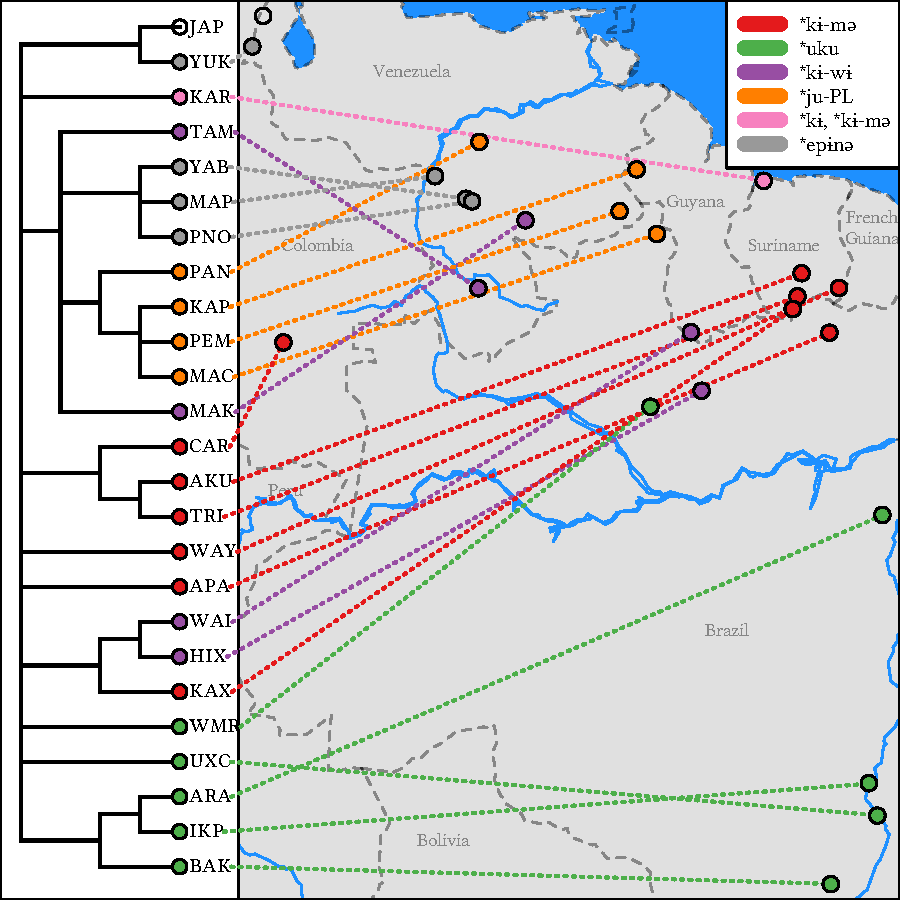
\includegraphics[width=0.7\textwidth]{images/1+2_map.pdf}
	\caption{Geographical and genealogical distribution of \gl{1+2} cognates}
	\label{fig:12}
\end{figure}

\begin{table}
\centering
\caption{Distribution of grammaticalized emphatic markers}
\label{tab:empstats}
\begin{tabular}[t]{@{}lrrr}
\mytoprule
                    Pronoun &  With \gl{emp} &  Total &  Ratio \\
\mymidrule
                     \gl{2} &             20 &     24 & 83.33\% \\
         \gl{med}.\gl{anim} &             14 &     17 & 82.35\% \\
              \gl{2}\gl{pl} &             19 &     24 & 79.17\% \\
            \gl{1+2}\gl{pl} &             11 &     16 & 68.75\% \\
   \gl{3}.\gl{anim}.\gl{pl} &              8 &     12 & 66.67\% \\
 \gl{med}.\gl{anim}.\gl{pl} &              8 &     14 & 57.14\% \\
                   \gl{1+2} &              9 &     20 & 45.00\% \\
                     \gl{1} &             11 &     25 & 44.00\% \\
\gl{prox}.\gl{anim}.\gl{pl} &              7 &     20 & 35.00\% \\
        \gl{prox}.\gl{anim} &              4 &     20 & 20.00\% \\
\gl{dist}.\gl{anim}.\gl{pl} &              1 &     15 &  6.67\% \\
 \gl{prox}.\gl{inan}-\gl{1} &              1 &     16 &  6.25\% \\
         \gl{med}.\gl{inan} &              1 &     22 &  4.55\% \\
\mybottomrule
\end{tabular}
\end{table}

	
	% NEW COGNATES
%	\ikpeng \obj{oren} and \obj{wam} are from \rc{mətjə} and \rc{mətjə-jamo}
%	Manapiarean cognate with Yukpa? And what is relation to \gl{1+3}?
	
	%LOSS OF DISTINCTIONS
%	Pekodian has reflexes of everything except \gl{med}.\gl{anim}.
	
	% CLASSIFICATION
	A clear shared innovation in the pronominal system is the development of first person \rc{əwɨ} to \rc{ju} in \PPP.
	A potential additional criterion for the suggested Venezuelan branch \parencites{gildea2004classification}{mattei2002busca}{gildea2015venezuelan} is the loss of the initial syllable of \rc{məkɨ-rə} \qu{\gl{med}.\gl{anim}}, see \akawaio \obj{kɨrə}, \panare \obj{kən}, or the \maqui plural \obj{kanno} \parencites[85]{stegeman2014akawaio}[89]{panarepayne2013}[122]{maquiritaricaceres2011}.
	
	There are also potential contact effects: the southern Pekodian languages \bakairi and \ikpeng (but not more Northern \arara) share with \uxc the loss of initial \rc{m} in the same pronoun: \arara and \ikpeng \obj{mogɨn} and \obj{ugun} \qu{\gl{dist}.\gl{anim}} \parencites[72]{alves2017arara}[119]{ikpengpacheco2001}, \bakairi and \uxc \obj{akaemo} and \obj{akaɣo} \qu{\gl{dist}.\gl{anim}.\gl{pl}} \parencites{meiraDBbakairi}[55]{kuikurodossantos2007}.
Finally, \arara and \ikpeng \obj{ug(o)+ro+ŋmo} \qu{\gl{1+2}\gl{pl}} \parencites{souza1993arara}[119]{ikpengpacheco2001} etymologically correspond to \uxc \obj{kuku+ɣe+ko} \parencites[55]{kuikurodossantos2007}, though this may be a coincidence.
		
		 
	% CONTACT
	

	% PLURALS
	
	% INANIMATE PROXIMALS
	\newpage
	\printbibliography
\end{document}